% vim: set tw=78 tabstop=4 shiftwidth=4 aw ai:

\chapter{Proiectarea unui protocol Multiparty îmbunătățit în nucleul Linux }
\label{chapter:multiparty}

%\todo{BitTorrent limitations, TCP vs. UDP, LEDBAT, P2P streaming, uTP,
%uTorrent}

\section{Protocolul swift Multiparty}
\label{sec:multiparty:swift}

Protocolul \textit{swift} este un protocol multiparty generic de transport.
Scopul său principal este de a desemina conținut între peer-ii din swarm.
Practic răspunde la doar o singură cerere: \textit{'Uite aici hash-ul!
Dă-mi datele pentru el!}. Entități ca mediile de stocare, servere și
conexiuni sunt abstractizate și sunt invizibile la nivelul API-ului.
Dându-se un hash, datele sunt primite de la oricare sursă este dispoinibilă
și integritatea lor sunt verificate criptografic folosind arbori hash
Merkle \cite{merkle}.


%\todo{current implementation, TUDelft, Victor Grishcenko}

Dacă ai nevoie de niște date, este mai rapid și/sau mai ieftin să le
descarci de la o un duplicat bine provizionat, dar pe de altă parte, acest
proces necesită ca multe entități (ex. clienți, surse de date, situri CDN,
mirror-uri, peer-i) să fie coordonați. Cum continutul de pe Internet este
în continuă creștere, overhead-ul de cooronare a peer-ilor devine mai
costisior decât descărcarea propriu-zisă. Prin urmare, nisă pentru
trasnsferuri multiparty se extinde. Tehnologiile curente și relevante sunt
încă strâns legate cu un singur caz de folosire sau chiar la o
infrastructură specifică unei singure organizații. Acestea sunt motivele
pentru care protocolul \textit{swift} vine cu principalul scop de a fi un
portocol de transfer multiparty generic centrat pe conținut, ce permite
deseminarea aparent fără efort a datelor în marele nor reprezentat de
Internet.

Mare parte din facilitățile oferite de protocolul \textit{swift} sunt
definite de funcția sa de protocol de transport multiparty centrat pe
conținut. O diferență seminificativă între \textit{swift} și protocolul TCP
este faptul că TCP-ul nu deține nici o informație despre datele pe care le
transportă când datele sunt primite din user-space, pe când protocolul
\textit{switf} are date stabilite anterior și mulți peer-i participă la
distribuirea aceluiași set de date. Din acest motiv și din cauza faptului
ca pentru protocolul \textit{switf} ordinea recepționării informației are
puțină importanță 
TODO!!!!

Fiind implementat peste UDP, protocolul face tot posibilul să păstreze
independența fiecărei datagrame astfet încât fiecare datagramă să poată fi
porocesată separat și o pierdere de pachet să nu perturbe sever fluxul de
date. Astfel, o datagramă conține unul sau mai multe mesaje iar un mesaj
sau dependențele lui nu ar trebui să fie trimis peste mai multe datagrame.

Verificarea bucătilor de date este realizată folosind un arbore de hash
Mekle \cite{merkle}, integrat ca o extensie în BitTorrent
\footnote{\url{http://bittorrent.org/beps/bep\_0030.html}}. Acest lucru
înseamnă că toate hash-urile necesare pentru validare integrității
trebuiesc să fie plasate în aceeași datagramă ca și datele corespunzătoare.
În ambele cazuri de folosire, streaming și downloading, o schemă comună de
verificare a inegrității, ce funcționează până la nivelul unei singure
datagrame, este dezvoltat.Ca o regulă generală, trimițătorul ar trebui să
atașeze datelor un set de meta-date reprezentând hash-urile necesare pentru
verificarea inegrității. Deși niște optimizări optimiste sunt sigur
posibile, destinatarul ar trebuie să arunce pachetul dacă îi este impisibil
de validat. Înainte de a trimite un pachet de date destinatarului,
trimițătorul inspectează confirmările anterioare ale receptorului pentru a
vedea care hashuri sunt deținute sigur de receptor.

Primirea datelor este confirmată sub forma de intervale binare, cu
intervalul de bază de 1KB. Drept urmare, fiecare pachet este confirmat de
un număr logaritmic de dăți. Acest mecanism oferă o redundanță necesară a
confirmărilor și compensează suficent nefiabilitatea datagramelor.

Singura funcție din TCP care este la fel de critică pentru \textit{swift}
este controlul congestiei. Pentru a facilitate controlul congestiei pe bază
de întârziere, o confirmare conține, pe lângă dimenziunile fișierului primit
de la transmițător, și un timestamp.

Principalul nostru obiectiv este integrarea protocolului \textit{swift} ca
un protocol de transport în stiva de rețea din nucleul Linux. Acest lucru
va crește semnificativ performanța transferurilor de date. Dorim să facem
acest lucru cu o intruziune minimă asupra nucleului Linux și modificând cât
mai puțin implementarea actuală de \textit{swift}. Un alt scop este de crea
un API transparent între nucleu și user-space. Un dezvoltator va folosi o
interfață de tip socket pentru a construi o aplicație peste protocolul
\textit{swift}. Pentru a îndeplini acest scop, am implementat un pas
intermediar. Am simulat bucata din kernel în user-space folosind socket-i
raw. Acest lucru are avantajul de a pune la dispoziție o metodă modulară de
a testa funcționalitățile.

%\todo{binmaps}
%\todo{stadardization}

\section{Proiectarea unui Protocol Multiparty}
\label{sec:multiparty:design}

%\todo{based on swift}
%\todo{decisions: user-space, kernel-space}
%\todo{phases: preliminary, raw sockets}
%\todo{possibilities: socket interface, netlink sockets, device interface}
%\todo{compatibility with socket interface}

În proiectarea sistemul nostru, am încercat diverse idei, fiecare cu
avantajele și dezavantajele ei. Vom prezenta unele dintre ideile
preliminare ce au condus la alegerea variantei finale.

Prima abordare la care ne-am gândit a fost să includem toate componentele
protocolului swift în nucleu. Acest lucru avea avantajul simplității și ar
fi însemnat un minim de schimbări în arhitectură. Implementarea actuală de
user space putea fi portată ca un modul de kernel.

Deși simplă, această abordare nu putea fi implementată din cauza
restricțiilor de mărime a memoriei în kernel. Pentru testulde integritate,
protocolul swift folosește arbore de hash Merkle. Păstarea acestui arbore
în memoria nucleului nu este scalabilă. Conținutul de pe Internet este mult
prea mare pentru a fi stocat în kernel space. Chiar dacă arborele reține
doar hash-urile datelor deseminate, spațiul tot este insuficient.

\begin{figure}
  \centering
  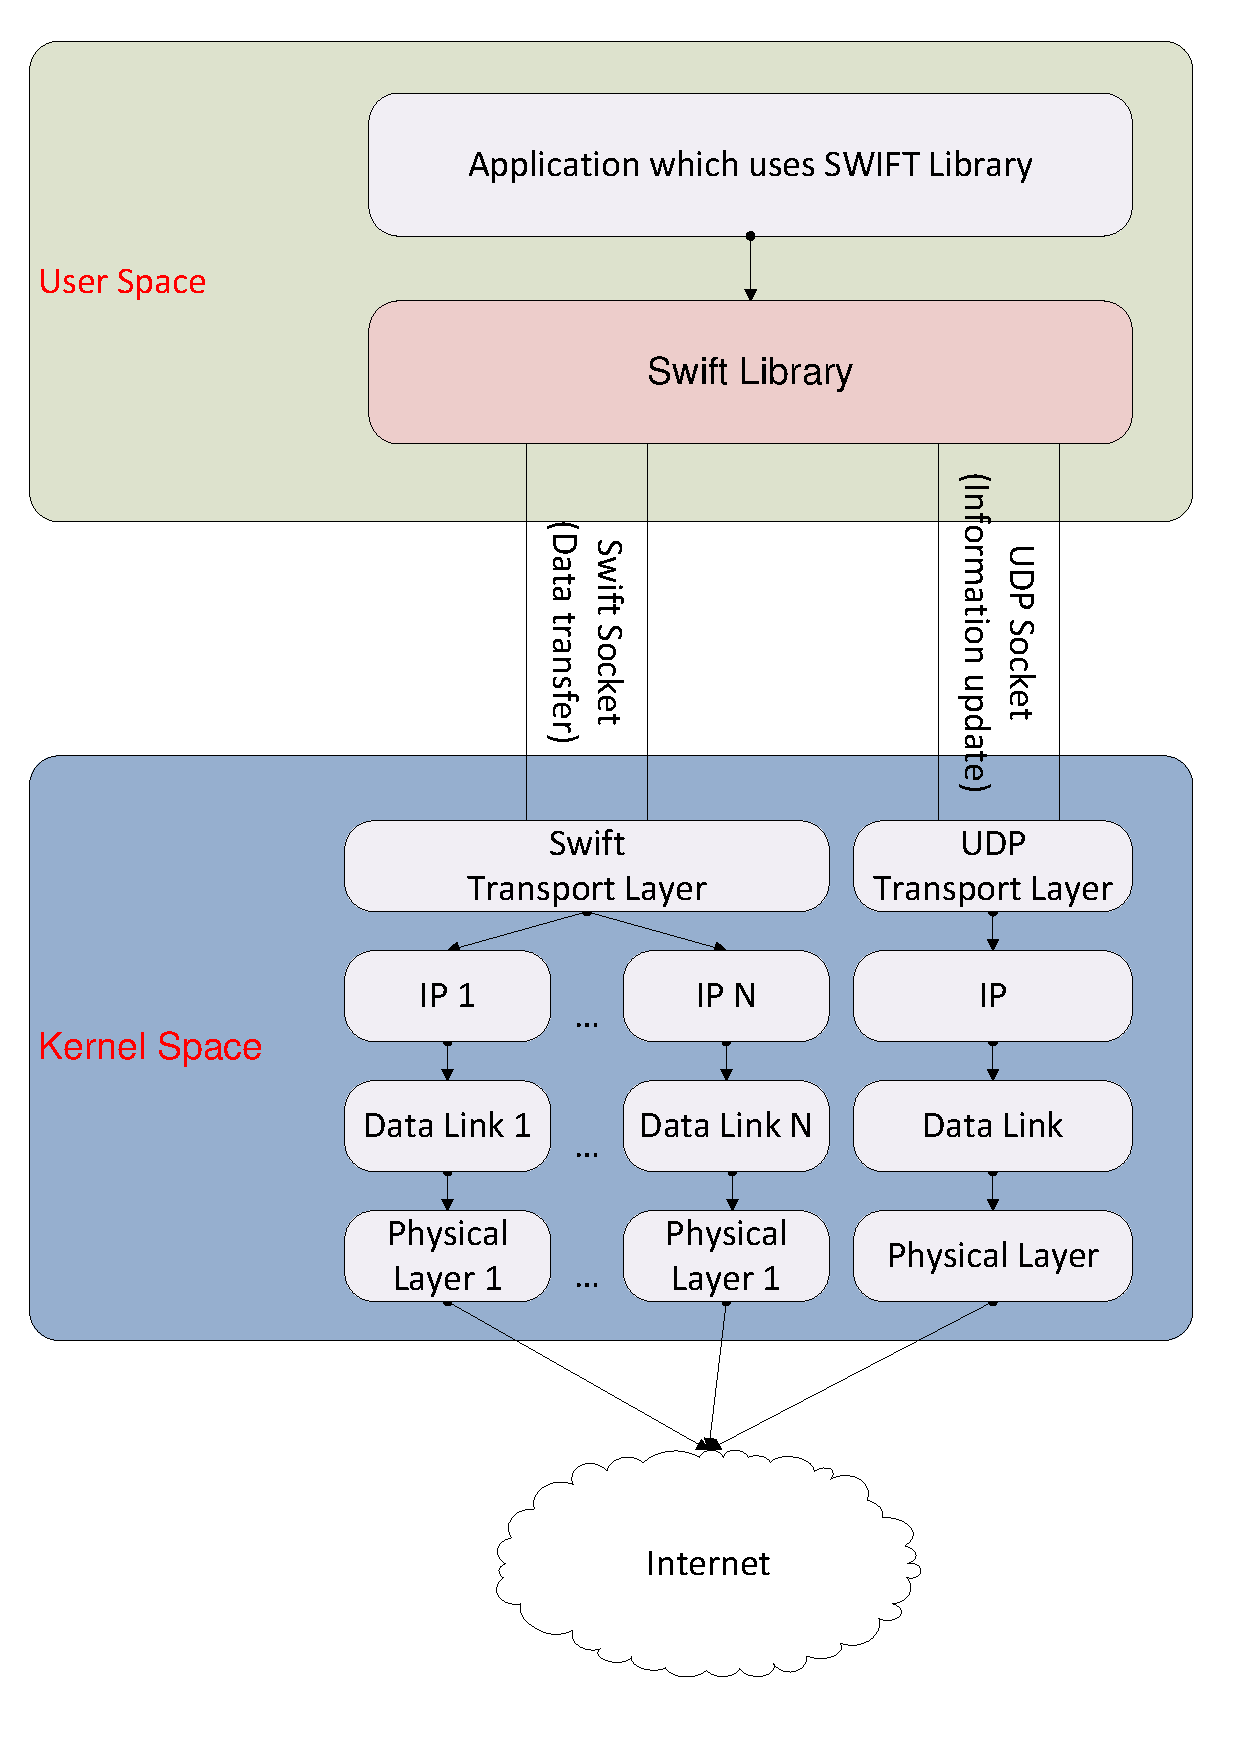
\includegraphics[width=0.4\textwidth]{src/img/multiparty/preliminary-architecture}
  \caption{Preliminary Architecture}
  \label{fig:multiparty:preliminary-architecture}
\end{figure}

A doua idee pentru implementarea protocolului swift este reprezentată în
figura~\ref{fig:multiparty:preliminary-architecture}. Protocolul de
transport swift ar trebui să aiba o nouă interfață în nucleu care să
permită creerea de socket-i speciali de tip swift. Ar fi trebuit să
implementeze protocolul multiparty ce permite transportul bucăților de date
de la și spre stații într-un mod peer-to-peer.

Această implementare ar trebui să aibe cozi de cereri specializate și
cozi de metadate spre și dinspre user space. Un apel de sistem specificat
în API ar fi trebuie să permită aplicațiilor de user space să
interacționeze cu cozile sus menționale și, deci, cu implmentarea
protocolului multiparty.

Diferențe arhitecturale față de o cumunitație unu-la-unu precum TCP sua UDP
înseamnă că apelul de sistem nu ar fi urmărit paradigma clasică de
transmisie/recepție. Pentru a compensa acest fapt și pentru a pune la
dispoziție o interfață mai prietenoasă aplicațiilor din user space, o
bibliotecă a fost proiectată. Descoperirea peer-ilor și a bucăților de date
ar fi trebuit să fie responsabilitatea aplicației din user-space.
Biblioteca SWIFT ar putea să pună la dispoziție și wrapper-e peste un canal
de descoperire bazat pe UDP.

Hash-urile Merkle ar fi fost stocate și calculate în userspace. Această
abordare nu putea fi implementată din cauza restricției implementării
bibliotecii (ex. structura unei aplicații a utilizatorului ar fi prea
restricivă). Mai mult, implementarea nucleului ar fi trebuit să fie ca un
UDP cu suport de transfer multicast.

A treia abordare pentru implementarea swift a fost detașarea nivelului de
transport din implementarea originală a protocolului. Când am început
implementarea acestei idei, am găsit multe inconveniențe precum ar fi
duplicat mare parte din codul aplicației, nu puteam implementa un protocol
de descoperire și, iar, implementarea din nucelui ar fi trebuie să fie
similară cu un multicast-UDP.

Aceasă abordare nu ar fi putut fi implementată din cauză complexității
managementului nivelului de transport. Mai mult, nu am găsit destule
avantaje care să confirme că această implementare este mai bună decât cea
originală.

\section{Raw Socket Wrapper Implementation}
\label{sec:multiparty:raw-socket}

%\todo{why new architecture}

\subsection{Raw Socket-Based Architecture}

In this section we present a proposed architectural design along with the
motivation of choices. We are also going to detail the protocol and the packet
structure used.

In figure Figure~\ref{fig:multiparty:architecture-overview} we see the main
conceptual modules: Application module, wrapper library, peer discovery
overlay and the swift transport protocol layer.

\begin{figure}
  \centering
  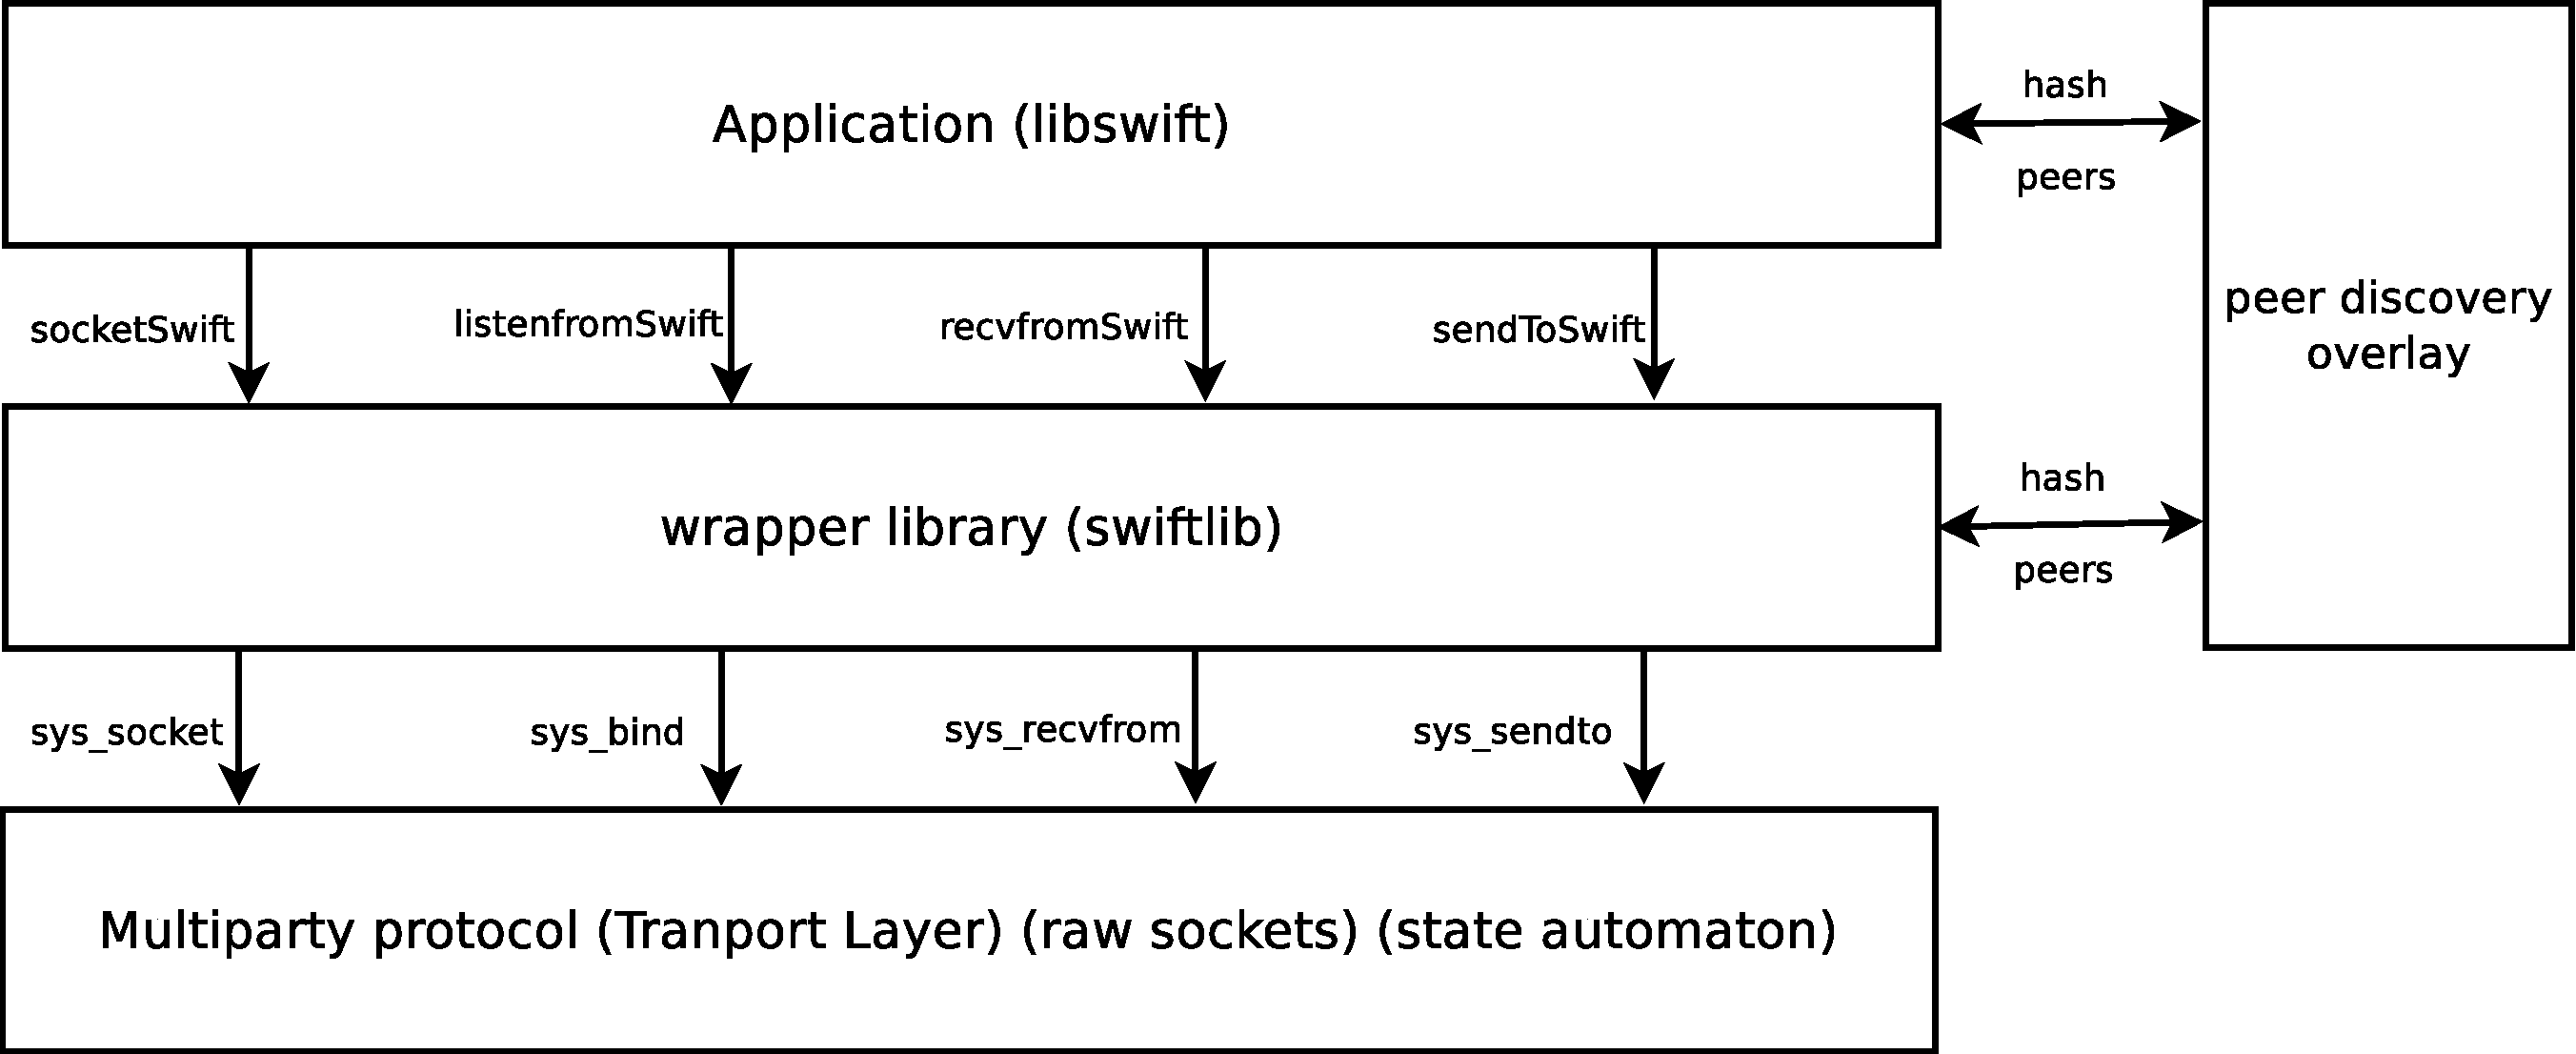
\includegraphics[width=0.6\textwidth]{src/img/multiparty/architecture-overview}
  \caption{Overview Architecture}
  \label{fig:multiparty:architecture-overview}
\end{figure}

The Application module represents the remaining part of the old swift
implementation. This is the part that remains in user space and contains the
file management and hash management features. 

The wrapper library module defines a socket-like API for the user space
applications. A regular program will use those calls instead of the normal
socket ones to use the multiparty sockets. For the moment those calls are
simulated system calls that initially are resolved with the socket raw
implementation (still in user space). In the future this wrapper library
will represent entry points into the kernel.

The peer discovery overlay will remain unchanged. It is still going to work
based on UDP sockets and link the same levels in the swift implementation as
before. The peer discover will be part of the application implementation and
it will be the developer's choice how to implement and how to manage it.

The multiparty protocol is implemented for now at user space level through a raw
socket layer to validate our architecture. This has the advantage of
simulating the real design modularization but also permits an easier debugging
and testing procedure of the integration. In the next step this part will be
represented by a kernel patch that will communicate through custom made system
calls with the wrapper library. This two phases are described in
Figure~\ref{fig:multiparty:detailed-architecture}.

\begin{figure}
  \centering
  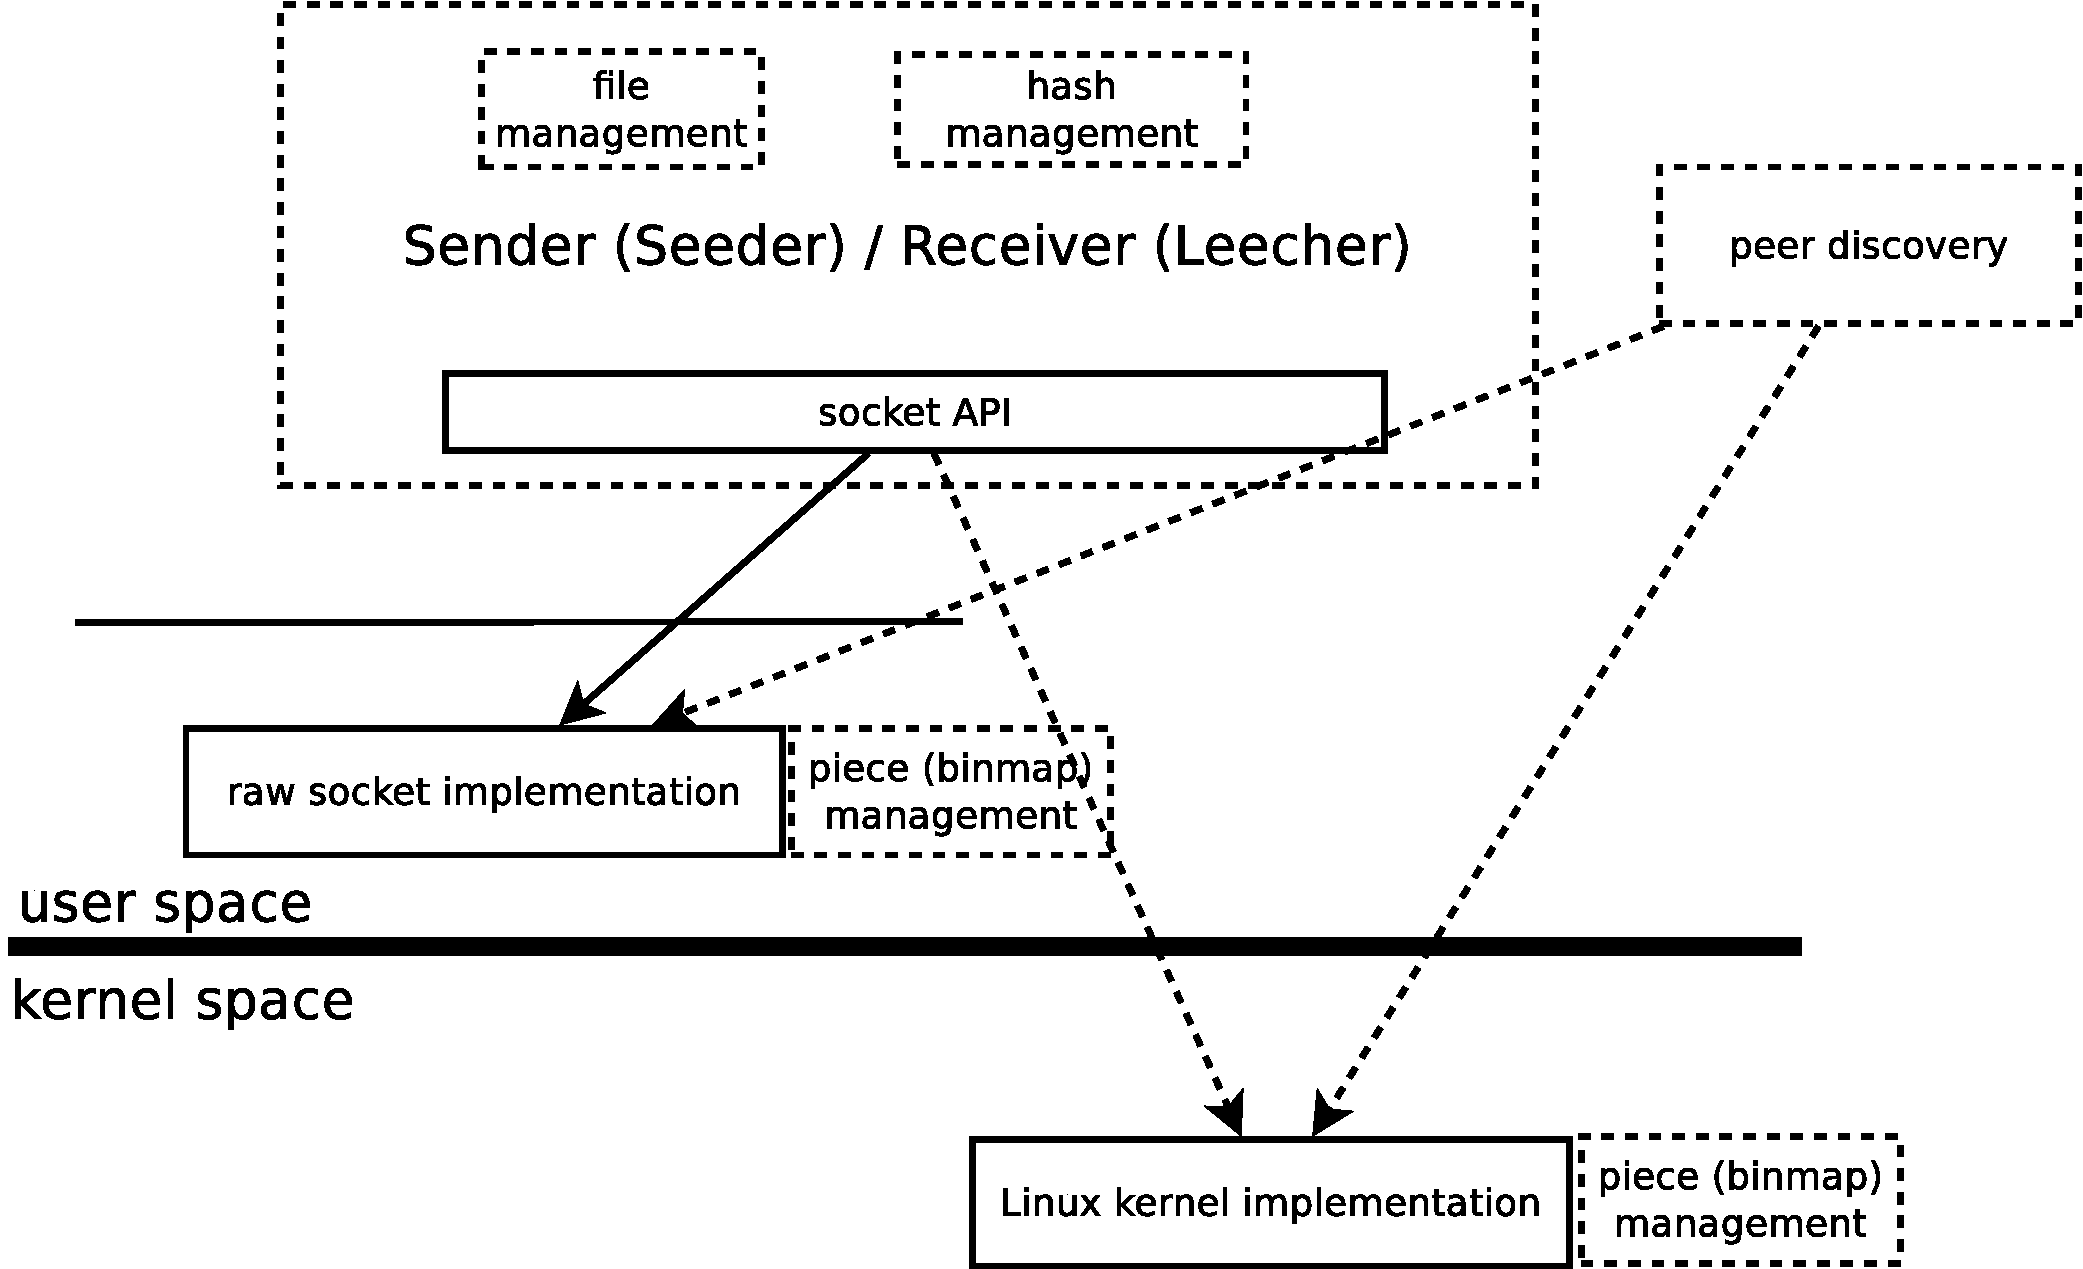
\includegraphics[width=0.6\textwidth]{src/img/multiparty/detailed-architecture}
  \caption{Detailed Architecture}
  \label{fig:multiparty:detailed-architecture}
\end{figure}

A socket is one of the most fundamental technologies of computer networking.
Sockets allow applications to communicate using standard mechanisms built into
network hardware and operating systems.

Raw mode is basically there to allow you to bypass some of the way that your
computer handles TCP/IP. Rather than going through the normal layers of
encapsulation/decapsulation that the TCP/IP stack on the kernel does, you just
pass the packet to the application that needs it. No TCP/IP processing -- so
it's not a processed packet, it's a raw packet. The application using
the packet is now responsible for stripping off the headers, analyzing the
packet, all the stuff that the TCP/IP stack in the kernel normally does for
you.

Raw socket implementation will support all system calls and it will be a copy of
the kernel implementation. This implementation will use the same API and
behavior as the kernel implementation. Still, in the first implementation, a
swift socket will be available to act as only a seeder or a leecher;
only one will be explicitelly supported: transmit data or receive data.

In the future implementation the swift protocol will be developed in kernel
space, and it will be accessible through a datagram socket that will support
all socket syscalls. It will intend to support both data operations (receive
and send) over a single socket.

\begin{figure}
  \centering
  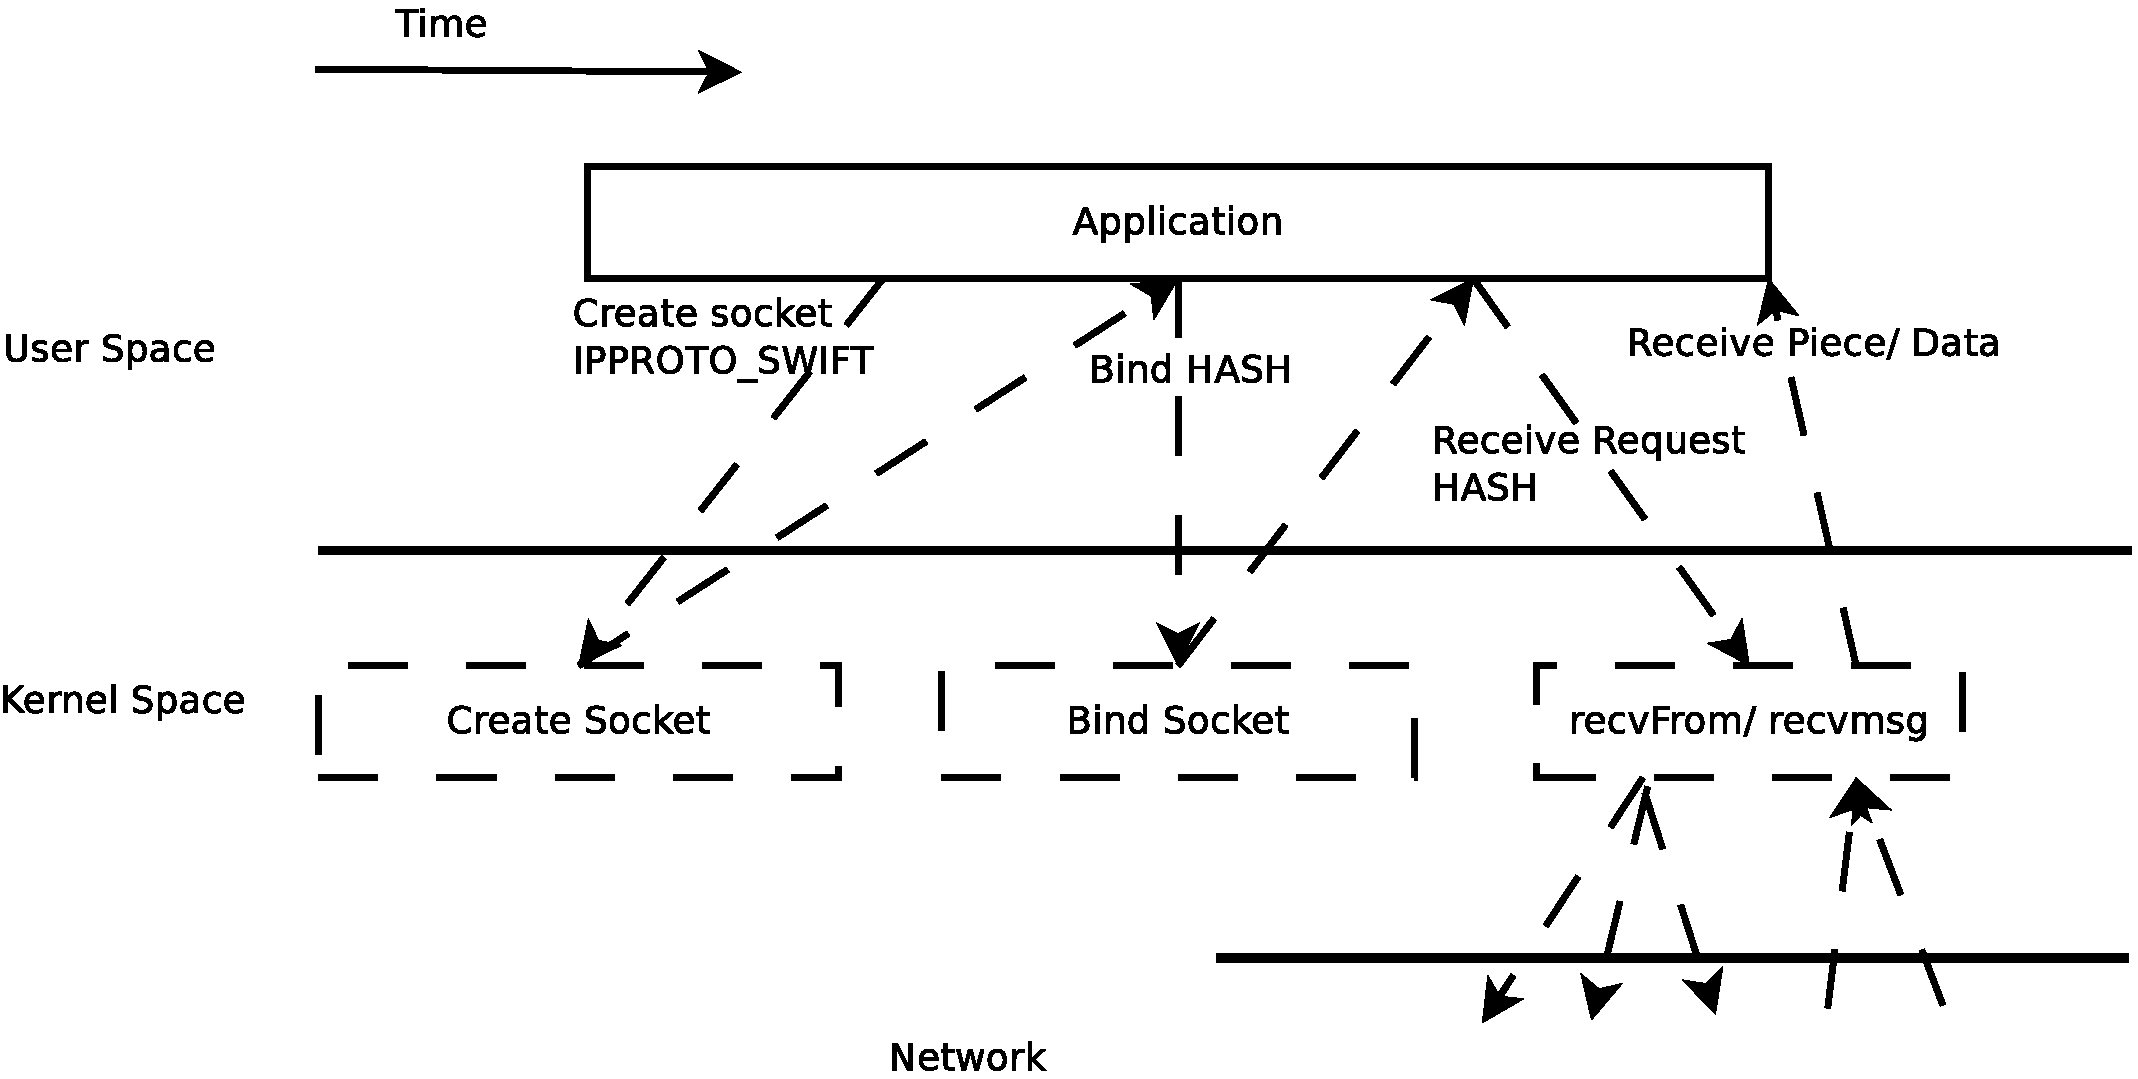
\includegraphics[width=0.55\textwidth]{src/img/multiparty/multiparty-recvmsg}
  \caption{Receiver Conceptual Model}
  \label{fig:multiparty:multiparty-recvmsg}
\end{figure}

Figure~\ref{fig:multiparty:multiparty-recvmsg} presents the conceptual model
of the Leecher. The Leecher is the one that requests data data. In order
to do this it must connect to the multiparty protocol by creating and binding
to a multiparty socket. When it binds to a socket, it uses the hash as a
parameter to find a connection with a peer that accesses the respective file.
This discovery is done through the separate peer discovery overlay. The
Leecher then waits for packets from seeders.

\begin{figure}
  \centering
  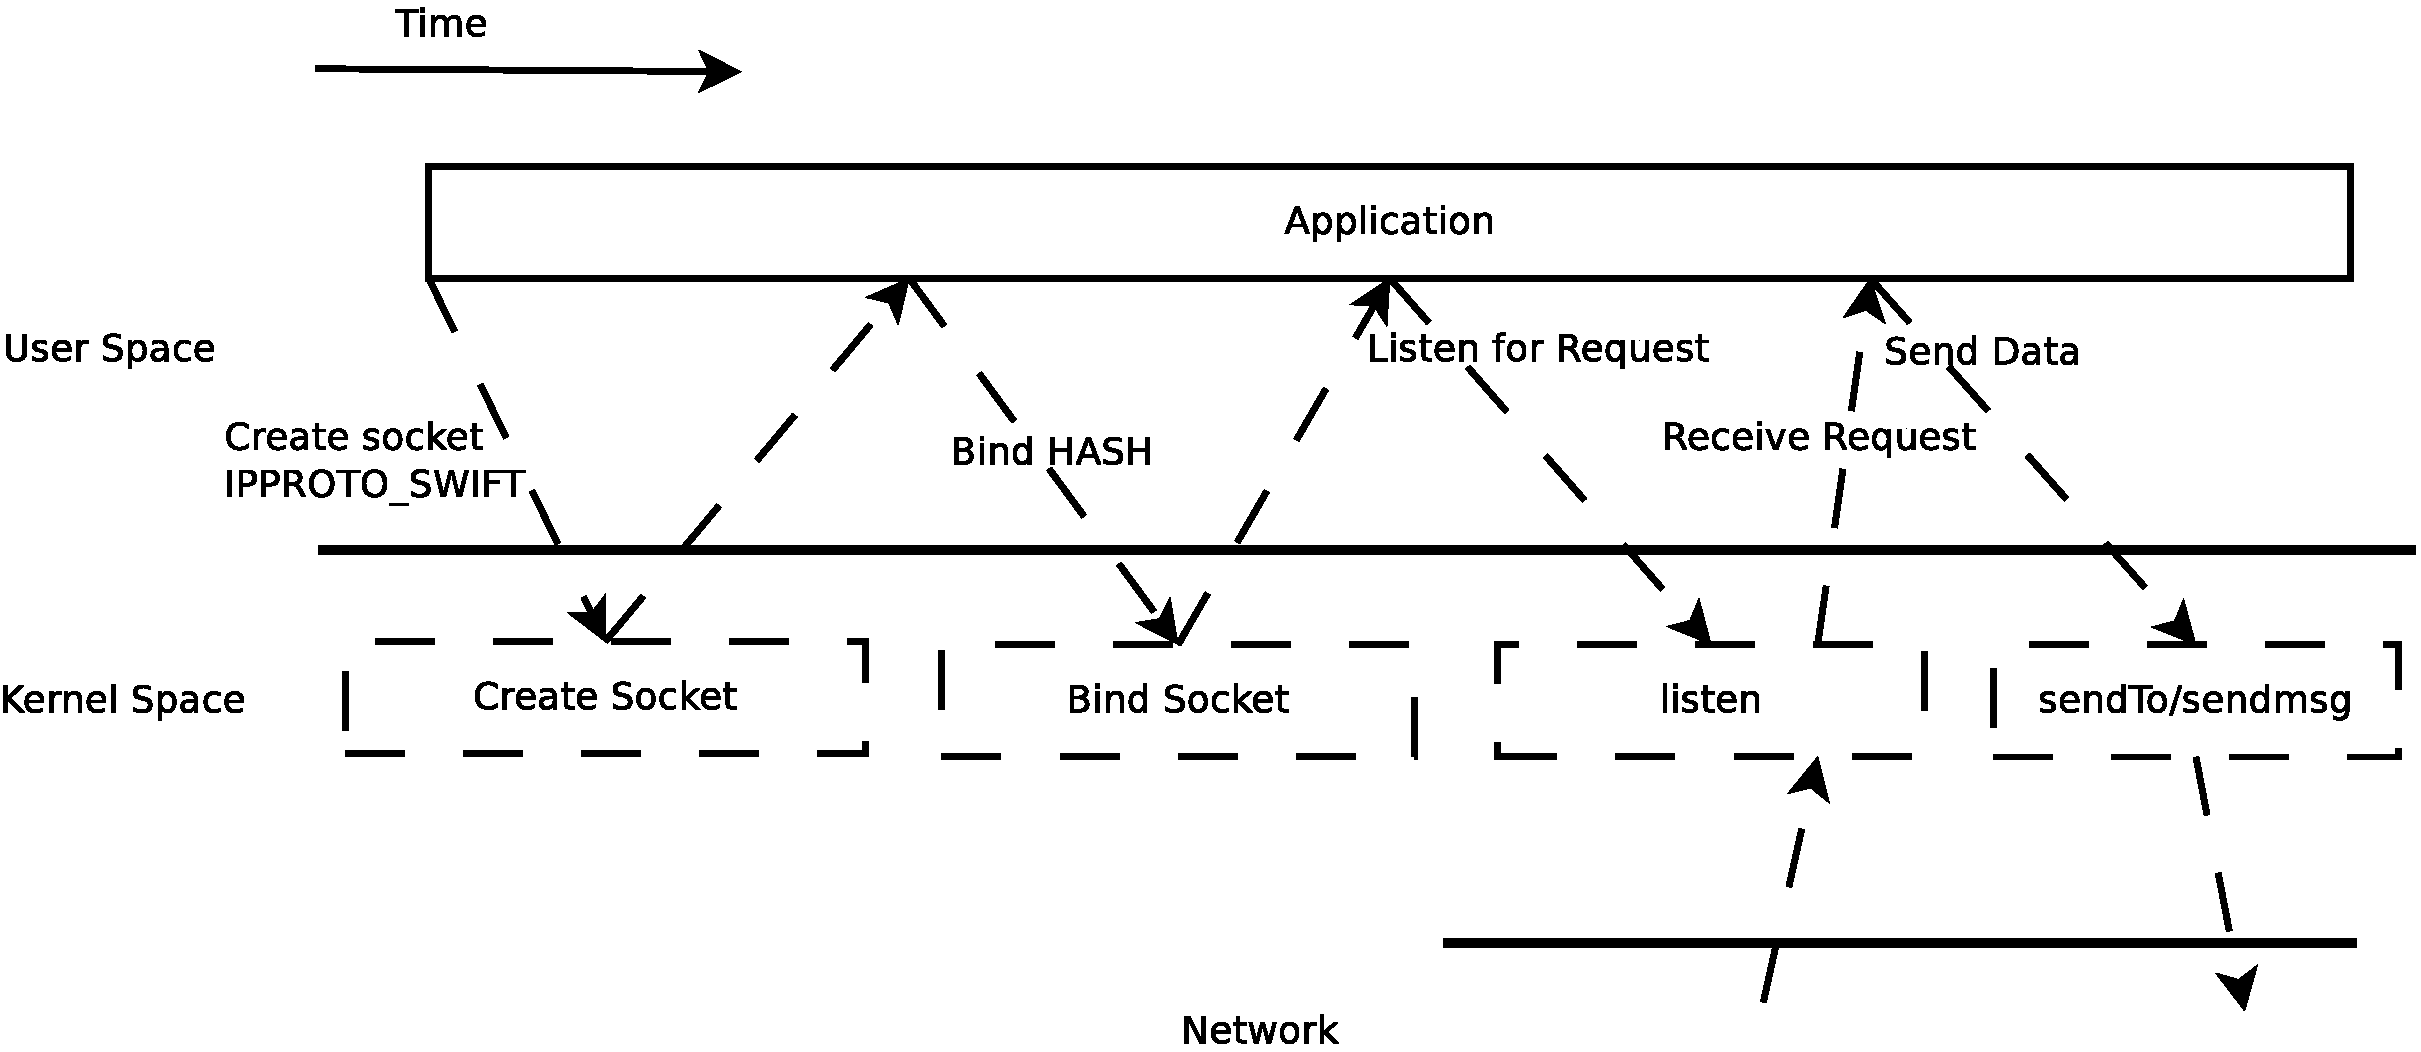
\includegraphics[width=0.55\textwidth]{src/img/multiparty/multiparty-sendmsg}
  \caption{Sender Conceptual Model}
  \label{fig:multiparty:multiparty-sendmsg}
\end{figure}

Figure~\ref{fig:multiparty:multiparty-sendmsg} presents the conceptual model
of the Seeder. The Seeder is the one that serves data to other Leechers. In
order to do this it must connect to the multiparty protocol by creating,
binding and listening to a multiparty socket. When binding, the Seeder
uses the hash as a parameter. This means that for every file hashed there will
be a socket on which the seeder that may receive and serve requests. The Seeder
then waits for requests and sends data packets as requested.

\subsection{Testing of Raw Socket Implementation}

The  protocol is a generic multiparty transport protocol. Its mission is to
disseminate content among a swarm of peers.  Given a hash, the data is
received from whatever source available and data integrity is checked
cryptographically with Merkle hash trees. 

Our main focus when modifying the swift implementation is to have an impact on
time performance. With a communication protocol the greatest latency is
usually generated by waiting for the results from the network. The multiparty
communication model already takes care of this, so the next best thing is to
enhance the application time. We are doing this by decreasing time
penalties due to context switches between user space and kernel space. The
main idea is to reduce the number of system calls made from user space into
the kernel. This implicitly reduces the number of preemption moments.

First, we have implemented a test suite for every socket system call, which
tests all possible cases. These unit tests are created to ensure the code
quality, and to validate if the system call behave in the same mode as other
similar system call.

Secondly, we have implemented a functional test suite to validate a simple
workflow. For this purpose we tested a peer that acts as the seeder and a
receiver which behaves as a leecher. A small file is transfered between the
two entities to ensure proper delivery.

The test suite is mainly implementing using arrays of function pointers or
function pointer structures. A top level structure defines test suites for
each function exported by the implementation. Each test suite is a series of
methods that test a variant of the call of the function.

The top-level test suite is defined by the \texttt{test\_fun\_array} as seen
in Listing~\ref{lst:multiparty:test-fun-array}.

\lstset{language=C,caption=Test Suite Top-Level
Array,label=lst:multiparty:test-fun-array}
\begin{lstlisting}
static void (*test_fun_array[])(void) = {
    NULL,
    test_dummy,
    socket_test_suite,
    bind_test_suite,
    getsockname_test_suite,
    getsockopt_test_suite,
    sendto_test_suite,
    recvfrom_test_suite,
    sendmsg_test_suite,
    recvmsg_test_suite,
    close_test_suite,
};
\end{lstlisting}

Each member of the array is a test suite for the functions exported by the
implementation. Exported functions are basic socket API functions. Each such
test suite is a sequentiall caller of individual test methods, as shown in
Listing~\ref{lst:multiparty:recvfrom-test-suite}.

\lstset{language=C,caption=Test Suite for recvfrom Call,label=lst:multiparty:recvfrom-test-suite}
\begin{lstlisting}
void recvfrom_test_suite(void)
{
    start_suite();
    recvfrom_dummy();
    recvfrom_invalid_descriptor();
    recvfrom_descriptor_is_not_a_socket();
    recvfrom_socket_is_not_bound();
    recvfrom_after_sendto_ok();
    recvfrom_after_sendmsg_ok();
}
\end{lstlisting}

Each individual method is used to test a single aspect of the test suite. For
example, the \texttt{recvfrom\_socket\_is\_not\_bound} shown in
Listing~\ref{lst:multiparty:recvfrom-socket-is-not-bound} tests the
implementation for sending out an error when receiving from a socket that is
not bound (that is no \texttt{bind} call was provided).

\lstset{language=C,caption=Basic Method for Testing recvfrom
Call,label=lst:multiparty:recvfrom-socket-is-not-bound}.
\begin{lstlisting}
static void recvfrom_socket_is_not_bound(void)
{
    int sockfd;
    struct sockaddr_sw local_addr;
    struct sockaddr_sw remote_addr;
    ssize_t bytes_recv;
    char buffer[BUFSIZ];

    sockfd = sw_socket(PF_INET, SOCK_DGRAM, IPPROTO_SWIFT);
    DIE(sockfd < 0, "sw_socket");

    fill_sockaddr_sw(&local_addr, &remote_addr, "127.0.0.1", "myHash", "127.0.0.1");
    bytes_recv = sw_recvfrom(sockfd, buffer, BUFSIZ, 0, (struct sockaddr *) &remote_addr, sizeof(remote_addr));

    test( bytes_recv < 0 && errno == EAFNOSUPPORT );
}
\end{lstlisting}

We will implement performance tests that will validate our design and
implementation. These tests will compare the number of system calls for both
implementations (original swift implementation and our kernel based
implementation).

\section{Kernel Framework for Multiparty Protocol Implementation}
\label{sec:multiparty:kernel-framework}

The introduction of a multiparty protocol in the Linux kernel was a challenge,
because of its particularities versus common protocol implementations. A
multiparty transport protocol uses multiple points in a communication, unlike
a traditional communication protocol that allows a sender endpoint and a
receiver endpoint.

A traditional Transport Layer protocol header uses a port to differentiate
between various processes that take part in a communication and use Network
Layer address information for host information. For a multiparty Transport
Layer protocol, the port information would be substituted by a file. While
traditional protocols use ``data'' (either streams -- TCP, or datagrams --
UDP), a multiparty protocol is concerned about sending and receiving parts of
a given file, which significantly alters its design.

Currently, the swift protocol\footnote{\url{http://libswift.org}} that forms the
basis of the current design is implemented in user space, using UDP sockets.
There is no need for TCP, as ordered delivery offered by TCP is of no
importance to swift.  Packets may be received out of of order and the same
piece of information may be received multiple times from different peers.
Redundancy is important to swift: the first arriving piece is added to the
``stream'' while the rest are discarded.

The main feature of the swift protocol is that it's content-centric, unlike
TCP that possesses no knowledge of the transported data. Data possesses
meaning for swift.

Checking pieces that are received through swift is accomplished through the
use of Merkle hash trees. This means that all information
regarding integrity checking is already placed in the same data packet.

%\todo{focus on it being a module}

\subsection{Transport Protocol Implementation on the Linux Kernel}

In order to implement o transport protocol in the Linux kernel, several design
phases must be established:

\begin{itemize}
  \item Defining \texttt{IPPROTO\_\$\$}. This macro will identify the
  transport protocol. This will be subsequently used for creating a transport
  protocol socket.
  \item Defining a transport header. The framework we used defined two 8 bit
  ports, a source port and a destination port and a 16 bit lenght field. The
  latter field is the data length, including the tranport protocol header.
\end{itemize}

After the above have been completed, several data structures have to be
defined, as mentioned below.

A data structure that defines the new socket type. This is where we must save
information regarding the socket state, such as the destination or the source
port.
\begin{verbatim}
struct swift_sock {
    struct inet_sock sock;
    /* swift socket speciffic data */
    uint8_t src;
    uint8_t dst;
};
\end{verbatim}

The protocol definition, used by the socket, including its name and size are
defined in a \texttt{struct proto} structure.
\begin{verbatim}
static struct proto swift_prot = {
    .obj_size = sizeof(struct swift_sock),
    .owner = THIS_MODULE,
    .name = "SWIFT",
};
\end{verbatim}

The most important structure to be defined describes the operations that are
supported by a socket of a given type. For a datagram sending socket, the
implementation of \texttt{release}, \texttt{connect}, \texttt{sendmsg} and
\texttt{recvmsg} functions is sufficient.
\begin{verbatim}
static const struct proto_ops swift_ops = {
    .family = PF_INET,
    .owner = THIS_MODULE,
    .release = swift_release,
    .bind = swift_bind,
    .connect = swift_connect,
    .socketpair = sock_no_socketpair,
    .accept = sock_no_accept,
    .getname = sock_no_getname,
    .poll = datagram_poll,
    .ioctl = sock_no_ioctl,
    .listen = sock_no_listen,
    .shutdown = sock_no_shutdown,
    .setsockopt = sock_no_setsockopt,
    .getsockopt = sock_no_getsockopt,
    .sendmsg = swift_sendmsg,
    .recvmsg = swift_recvmsg,
    .mmap = sock_no_mmap,
    .sendpage = sock_no_sendpage,
};
\end{verbatim}

The new packtets header are setup in the \texttt{net\_protocol} header. New
packets that are received directly from the network will fill the
\texttt{protocol} field in the IP header with the value of the implemented
Transport Level protocol.
\begin{verbatim}
static const struct net_protocol swift_protocol = {
    .handler = swift_rcv,
    .no_policy = 1,
    .netns_ok = 1,
};
\end{verbatim}

A final data structure has to connect the new protocol to the operations on
the its socket. This structure uses two pointers to the \texttt{struct proto}
and \texttt{struct proto\_ops} data structures:
\begin{verbatim}
static struct inet_protosw swift_protosw = {
    .type = SOCK_DGRAM,
    .protocol = IPPROTO_SWIFT,
    .prot = &swift_prot,
    .ops = &swift_ops,
    .no_check = 0,
};
\end{verbatim}

As soon as the above structures are defined, the protocol defined will be
added to the kernel. The sequence of operations used to establish this step is
described below.

\begin{verbatim}
proto_register(&swift_prot, 1);
inet_add_protocol(&swift_protocol, IPPROTO_SWIFT);
inet_register_protosw(&swift_protosw);
\end{verbatim}

Before compiling and inserting the module in the kernel, several socket
operations functions have to be filled; for swift (a datagram based protocol),
this would mean \texttt{release}, \texttt{bind}, \texttt{connect},
\texttt{sendmsg} and \texttt{recvmsg}. A handler for packets received from the
network must also be implemented. At protocol level, one must keep a mapping
between a port and a socket, meaning that the socket is bound to that port.

Each implemented socket operation function fills different roles:

\begin{itemize}
  \item \texttt{release} is used fo freeing resources (most likely memory)
  used by the socket.
  \item \texttt{bind} checks the availability of the port and ties the socket
  to that port and a source IP address.
  \item \texttt{connect} maps the current socket to a destination port and IP
  address.
  \item \texttt{sendmsg} extracts the destination IP address and port,
  provided they were passed as arguments from user space. If they were not
  provided, the module checks whether the socket is connected (through a
  previous \texttt{connect} call), and, in case no socket is connected, error
  is returned.

  After establishing the receiving end (IP address and port), an
  \texttt{skb} structure is allocated, specifying the protocol header and the
  rest of the data. The swift header is filled, user space data are copied and
  the packet is routed. After the routing process, required data is copied and
  is queued for transmit using the \texttt{ip\_queue\_xmit} function call.

  \item \texttt{recvmsg} is responsible for the reverse operation of
  \texttt{sendmsg}. A datagram is read from the receiving queue through the
  use of the \texttt{skb\_recv\_datagram} call. Serveral integrity checks are
  employed, after which data is copied from the \texttt{skb} structure to user
  space.

  At the time, in case the sender address (IP address and port) has been
  requested (as used by the \texttt{recvmsg} and \texttt{recvfrom} socket API
  call), required information is filled in the user space buffer.

  In the end the \texttt{skb} structure is freed through the use of the
  \texttt{skb\_free\_datagram} call.

  \item The function passed as a handler in the \texttt{net\_protocol}
  structure is invoked when a packed is received. The protocol field in the
  packet IP header will be used to demultiplex the packet and call the
  required function.

  When the packet is received, several validations of this will take place.
  Subsequently, the destination port information will be extracted. A lookup
  operation returns the socked mapped to the destination port. The
  \texttt{skb->cb} field is initialized to information regarding the sender.
  Afterwards, the packed is added to the receive queue, through the use of
  \texttt{ip\_queue\_rcv\_skb}.
\end{itemize}

\subsection{Testing the Kernel Protocol Implementation}

Unit tests have been employed for testing the protocol. Among those are a few
simple tests, to ensure basic functionality and then a set of new tests that
check error codes and protocol performance. Protocol performance is related to
ensuring scalability -- multiple simulateneous client connections.

Basic functional testing means the design and implementation of tests for each
function exposed by the protocol. That is, there is a given test for each of
\texttt{bind}, \texttt{connect}, \texttt{close}, \texttt{sendto},
\texttt{recvfrom}, \texttt{sendmsg}, \texttt{recvmsg}, \texttt{send} and
\texttt{recv}. The test suite is used is the same one used for the raw
socket implementation. Due to the identical API provided, we could easily use
those test for the kernel implementation.

Negative testing, for unwanted/unwelcome situations is similarly accomplished:
each function exposed by the protocol is assigned a test. For example, the
\texttt{bind} system call will always check an error being returned for a
duplicate call using the same port. As is the case for the use of invalid IP
addresses or invalid port numbers. A series of such tests will be employed for
each functionality.

Performance testing is completed through the use of multiple protocol sockets.
Data sent from the socket is checked against data arriving at the other
end; this actually means checking whether port and socket mapping is working
according to the specifications. Another measure of protocol performance is
the transfer speed on the newly created socket.

\section{Conclusion}
\label{sec:multiparty:conclusion}

The \textit{swift} protocol is a multiparty content-centric protocol that aims
to disseminate content among a swarm of peers. This chapter proposes an
approach for the optimization of the currently \textit{swift} protocol. The
integration of communication in the kernel space as a multiparty transport
protocol that is solely responsible for getting the bits moving improves the
overall protocol performance. It ensures maximum efficiency of data transfer
by decreasing switches between user and kernel space and eliminating some
performance penalties due to those switches.

After we complete the implementation and the functional tests, we want to test
extensively our new features in a real environment. We plan to do stress tests
using a cluster. These tests will help create an overview about our
implementation and allow comparing against the user-space implementation of the
\textit{swift} to determine the encountered performance. If
results are satisfactory, optimization and feature addition are to be
continued.

It will be very useful to have a real application on top of the \textit{swift}
protocol. If not, one solution would be to port an application strictly for
this task. This would give us the opportunity to extend and refine our
implementation, and also to extend the library API.

The multiparty protocol is planned to be implemented in the Linux kernel, by
adapting it to the framework described above. By bringing the protocol to the
kernel, its performance should increase due to the decrease in the number of
user space/kernel space swiches (as part of the decrease of system calls).

Currently the framework lacks a packet fragmentation mechanism. The current
implementation can't send on a socket data larger then the \textit{Maximum
Transfer Unit} (\textit{MTU}) (1500 bytes for Ethernet). A possible solution
is borrowing the fragmentation mechanism used by the UDP implementation.
